\chapter{Evaluation}
\label{cha:evaluation}
This last chapter presents how the prototype have been evaluated to observe if and how it meets the initial research question.
Performance evaluation for the classifiers is presented. Then, Section~\ref{sec:InsAct} explains how the extracted insights can impact a business and help it in the interaction with its customers.

Classifiers for the four dimensions of the MBTI personality model were evaluated using confusion matrices.
A confusion matrix is a $2x2$ table used to observe the results of a binary classification algorithm.
In general, along its columns it contains the values predicted by the model. The rows represent the actual class of the samples. Figure~\ref{fig:confMat} shows how the table is structured.
The output of a binary classification can be either 0, or \textit{negative} class, or 1 \textit{positive} class.
So, the four cells of the matrix assume these names: at top-left, there is the \textit{true positives} (TP) counter, the top-right is the counter for the \textit{false negative} (FN), the bottom-left one for the \textit{false positives} (FP), and bottom-right for \textit{true negative} (TN).
Totally, their sum is equal to the number of samples classified.
From this table, four measures as usually extracted: 

\begin{equation*}
\begin{split}
\text{Accuracy} & = \frac{TP + TN}{TP + TN + FP + FN}\\
\text{Precision} & = \frac{TP}{TP + FP} \\ 
\text{Recall} & = \frac{TP}{TP + FN}\\
\text{F}_1\text{-Score} & = 2 * \frac{\text{Precision} * \text{Recall}}{\text{Precision} + \text{Recall}}
\end{split}
\end{equation*}

\begin{figure}
\centering
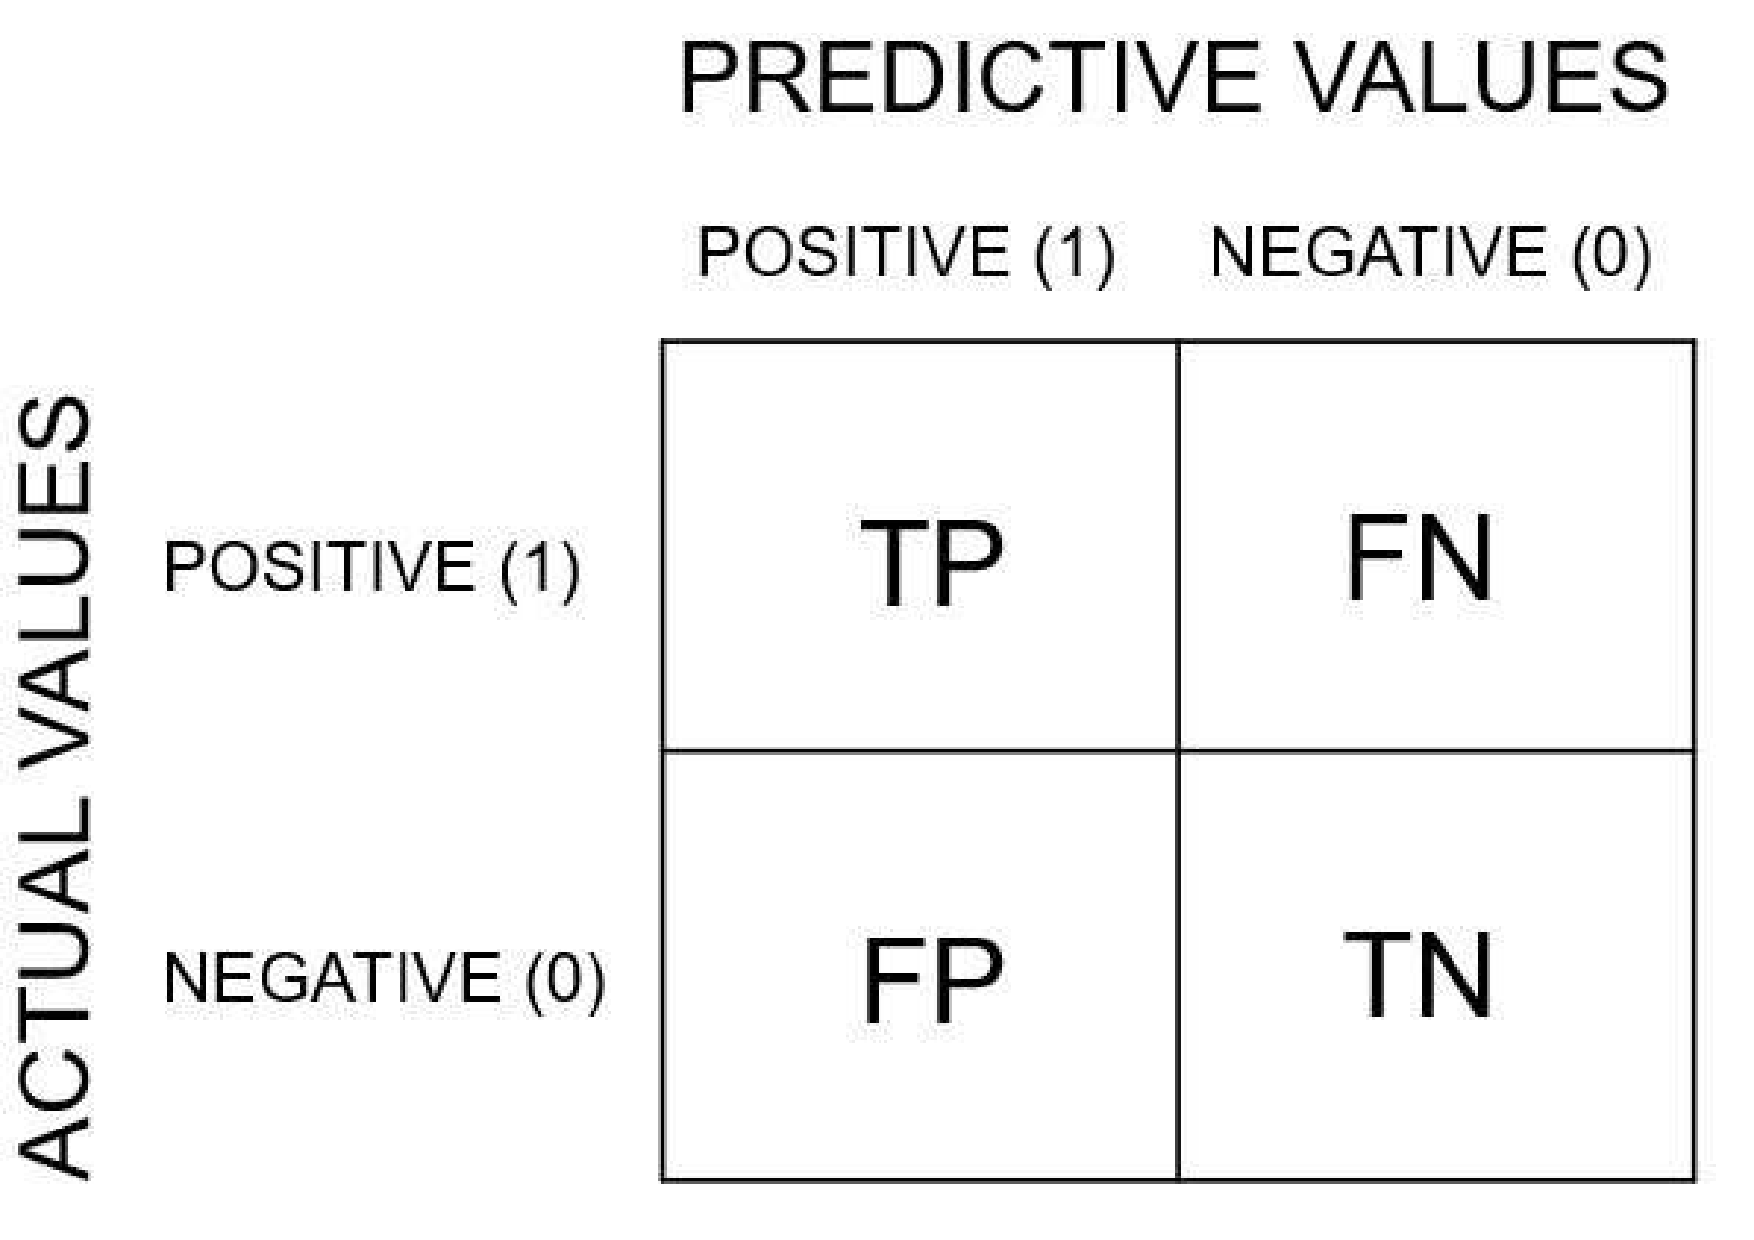
\includegraphics[width=%
0.7\textwidth,height=6.5cm,keepaspectratio]{img/confMatrix.pdf}
\caption{Generic schema of a confusion matrix}
\label{fig:confMat}
\end{figure}

\section{MBTI Classifiers evaluation}
Regarding these four classifiers, no particular setups have been applied.
Decision trees have been chosen as classifiers, according to the current state of the art.
Naive bayes classifiers are also usually applied for such purposes but were discarded due to bad performance with the linguistic features.

The performance evaluation has been computed on the same dataset used to train the four classifiers.
The dataset was split into a training set and a test one using the default values of the scikit-learn library. So, the training set contained $75\%$ of the samples and the test set the remaining $25\%$.
The used features include some information from the social profile, such as the number of followers and friends, the use of hashtags, mentions, and URLs, and other information describing the text component, such as the number of sentences and word and POS tags.
No particular configuration have been used for what regards \textit{bags of words} or \textit{n-grams}.

The measure observed to compare the performance with that of the current state of the art is the \textbf{accuracy}.
Accuracy is the ratio of correct prediction to total predictions made, presented as a percentage.
Accuracy is preferred since, for each of the four classifications, there is not discrimination between samples with a specific outcome from normal observation.
So, even though, taking as example the cognitive function \textit{Extroversion/Introversion}, extroversion is labelled as the negative class and introversion as the positive one, it is not the case where we want to reduce the number of false-positive rather than false-negative because both classes are treated the same way.
So, metrics such as precision or recall tend to be avoided and not considered in the state of the art.

Even though only standard methodologies have been applied, the classifiers had discrete results. 
Table~\ref{tab:results} compares the obtained results with that of the state of the art \cite{lima2019tecla}.
Compared to those obtained by Lima et al., the prototype's performances are slightly worse. 
It should be said that the study considered reached its best results using a particular set of psychological features extracted with services such as the \textit{Linguistic Inquire and Word Count} (LIWC).
But, as said in Section~\ref{sec:resObj}, this thesis focuses more on the actionability of the extracted insights rather than their accuracy and reliability.

\begin{table}[htbp]
    \centering
    \begin{tabular}{ccccc}
    \hline
    Classifiers & Extr/Intr & Sensation/Intuition & Think/Feel & Judging/Perceiving \\
    \hline
    \textbf{System accuracy} & $77.6\%$ & $81.8\%$ & $76.9\%$ & $74.3\%$ \\
    \textbf{SOA accuracy} & $82.0\%$ & $88.3\%$ & $80.57\%$ & $78.26\%$ \\
    \hline
    \end{tabular}
    \caption{Table.\label{tab:results}}
\end{table}

\section{Non-ML insights observation}
\label{sec:nonMLIns}
While for the four classifiers of the personality traits there is an availability of data for both the training and the evaluation of ML models, this is not possible for the other classifiers which are based on non-machine learning algorithms, described in Section~\ref{sec:Classifiers}.
To observe and evaluate their results, the user dashboard introduces in Section~\ref{sec:userDash} was used.

To do it, nearly twenty twitter profiles were downloaded and classified for a total of more than forty thousand activities.
Their results have been displayed over time thanks to the batch-based architecture and then observed individually.

Some interesting observations can be done comparing the results for two, or more, different profiles.
For example, two of the downloaded profiles, which comes from a similar environment, are the one of the \textbf{University of Trento} (\url{https://twitter.com/UniTrento}) and that of the \textbf{Department of Information Engineering and Computer Science} (\url{https://twitter.com/UniTrento_DISI}) show some interesting differences that deserve to be observed to understand better
at which point the system can actually be useful and usable. For each profile, the last two thousand activities have been fetched.
In Figure~\ref{fig:dailyComp}, the daily usage insights of these two profiles are compared.

First of all, it can be noticed that the two profiles tweet with different frequencies. Indeed, the last two thousand activities for the profile of the University of Trento covers 35 months, which brings to an average of 57 tweets per month, almost two per day. Differently, the same number of tweets ranges over 55 months for the Department of Information Engineering that corresponds to 36 activities per month and just over one tweet a month.
The latter also shows some months of no activity at all. During these periods the graph has no value and loses its continuity.

Then, looking at the values each graph has, we can observe that the two profiles differ much in terms of variability. 
The UniTN one is active especially during the afternoon, from 12:00 to 18:00, with some rare periods of morning activity.
On the other hand, the profile of the department fluctuates much more. It spreads its tweets particularly between morning and afternoon, so between 6:00 and 18:00. However, it also shows some activities at evening and night.

\begin{figure}
    \centering
    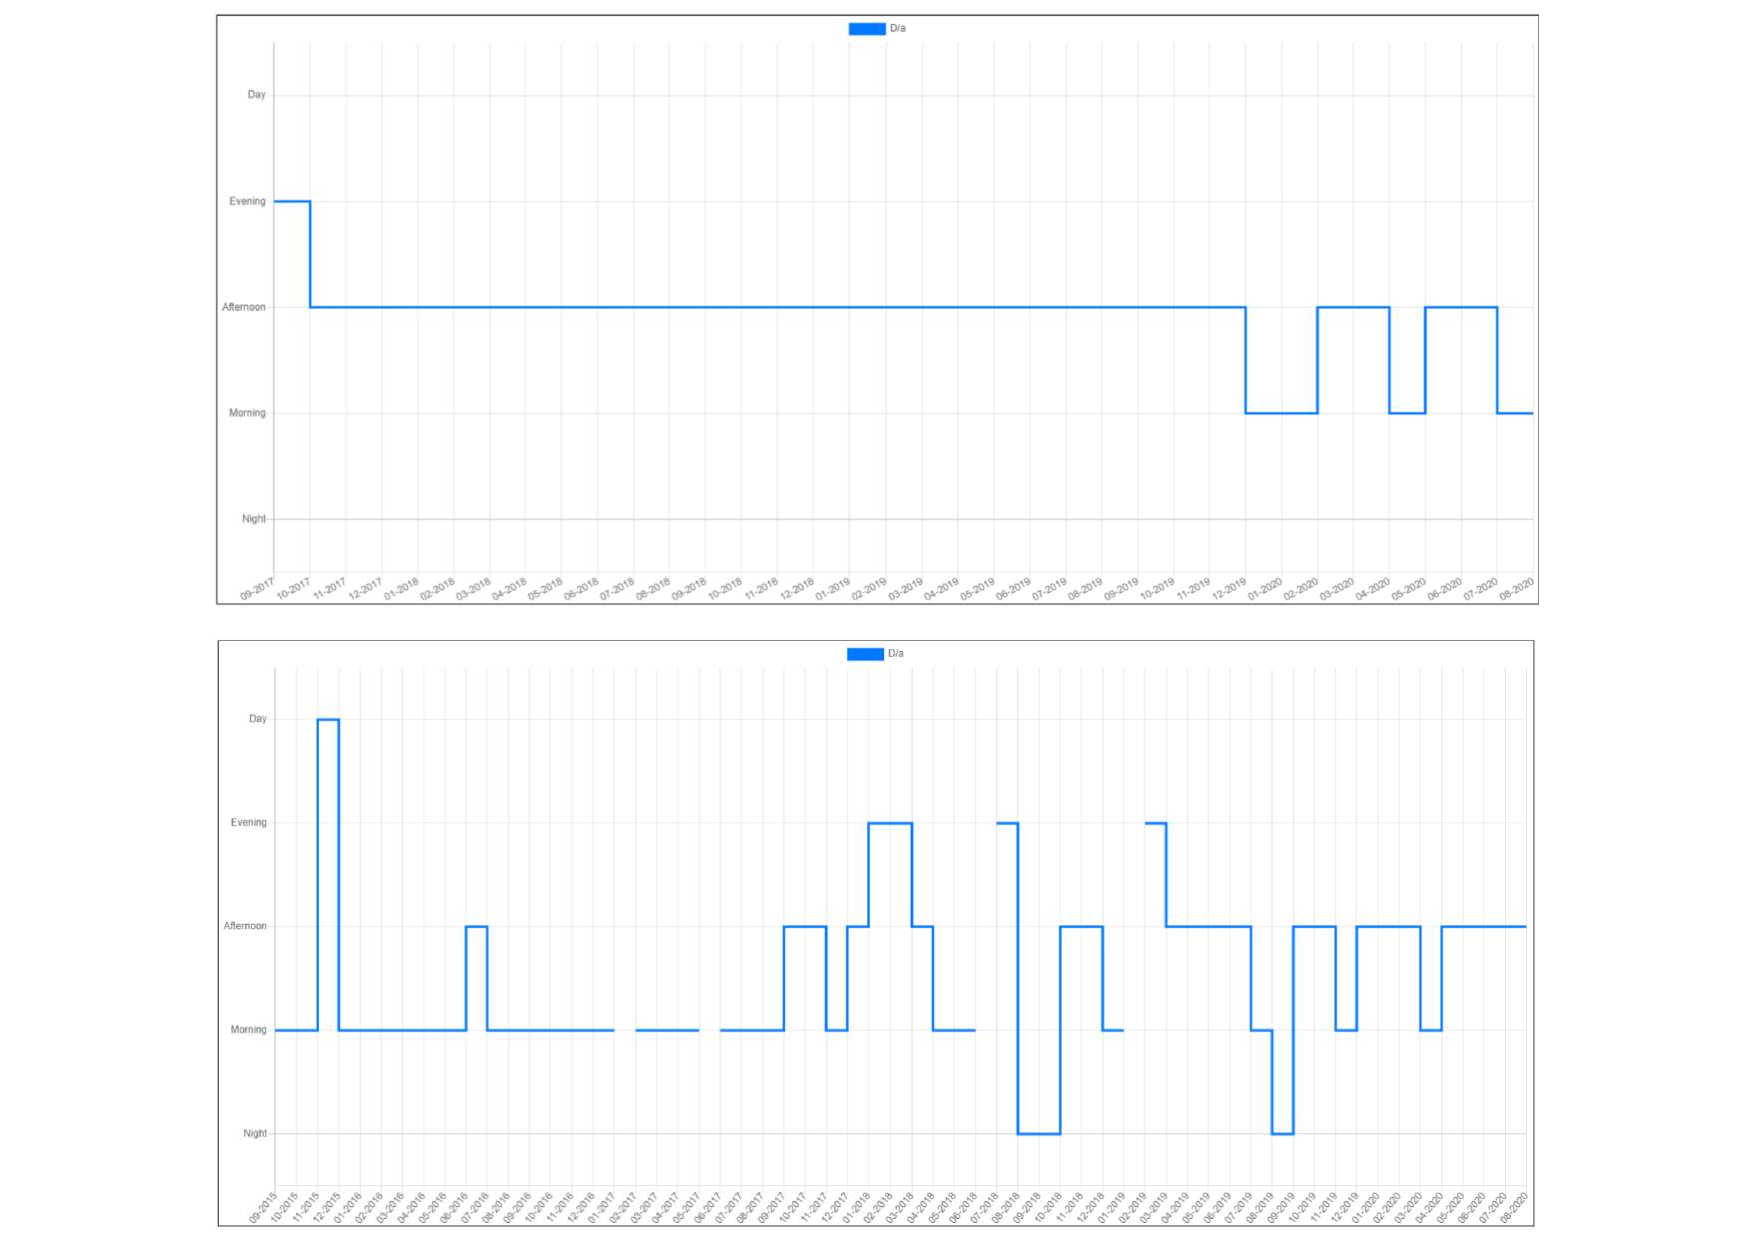
\includegraphics[width=%
    1.0\textwidth,height=14cm,keepaspectratio]{img/dailycomparison.pdf}
    \caption{Comparison between the \textbf{daily usage} insight of \textbf{UniTN}(1) and \textbf{DISI}(2)}
    \label{fig:dailyComp}
\end{figure}

One could use these types of comparisons to draw its conclusion in order to identify what's the difference between two or more profiles.
For example, in this case, we can assume that the University of Trento pays more attention to social reach, a metric that measures how many users came across its tweets. Indeed, it has been proved that the best time to post on Twitter is during the afternoon \footnote{\url{https://neilpatel.com/blog/is-there-a-generic-best-time-to-post-on-social-media-platforms/}}.
Contrarily, the profile of the department, which we can assume being more international rather than  national, does not have a particular time where the reach is higher; probably because of the different time zones of the followers.

The extracted attributes can then be observed in groups to find other correlations. Continuing with the example and the assumption about the internationality of the two profiles.
Observing and comparing the insights about the language in Figure~\ref{fig:langComp}, it can be said that the institute tends to talk only to their Italian students since their communications are done only in Italian while the department has to meet the language requirements of different nationalities and so English is highly preferred.
The previous example shows how the insights displayed by the system can help understanding a profile
\begin{figure}
    \centering
    \includegraphics[width=%
    1.0\textwidth,height=14cm,keepaspectratio]{img/langComparison.pdf}
    \caption{Comparison between the \textbf{language} insight of \textbf{UniTN}(1) and \textbf{DISI}(2)}
    \label{fig:langComp}
\end{figure}

\section{Insights' actionability}
\label{sec:InsAct}
An important goal that this thesis aimed to meet was to extract actionable insights. Insights capable of helping a company during their interaction with its customers.
This short section gives some examples of how the implemented classifiers can actually help a business.

Starting with the Extrovert/Introvert dichotomy, such information can be used, for example, in any marketing campaign to propose the customer a suited offer. For instance, introvert people may prefer something that does not involve any particular human relations while extrovert ones could be more attracted by group activities.

Some more obvious aspects are those regarding the language and daily usage of a person. The first one can be trivially useful to a company to relate with their customers with a specific language.
Then, the second characteristic can help the customer-company relation. Assuming that people tend to use social in their leisure, contacting them during these periods can encourage communications.

Differently from the previous ones, the insights about the communication style can also help adapting a particular service or product. For example, graphical interfaces may modify their views to completely satisfy the needs of each user. Indeed, someone could prefer images and videos while others like detailed pieces of text.

Moreover, the display of the results compared to time provided by the dashboard adds another degree of reading.
Indeed, taking as example the daily usage, it is easy to observe if there are patterns that repeat monthly.


